\documentclass{imsproc}
\usepackage{hyperref}
\newcommand*{\publname}{\begin{minipage}{\dimexpr(0.5\textwidth-0.5\columnsep-0.5\columnseprule)}
بیستمین سمینار آنالیز و کاربردهای آن%
\\[4pt]
۹ الی ۲۱ تیر ۱۳۹۰
\end{minipage}\hskip\dimexpr(\columnsep+\columnseprule)%
\begin{minipage}{\dimexpr(0.5\textwidth-0.5\columnsep-0.5\columnseprule)}
\raggedright
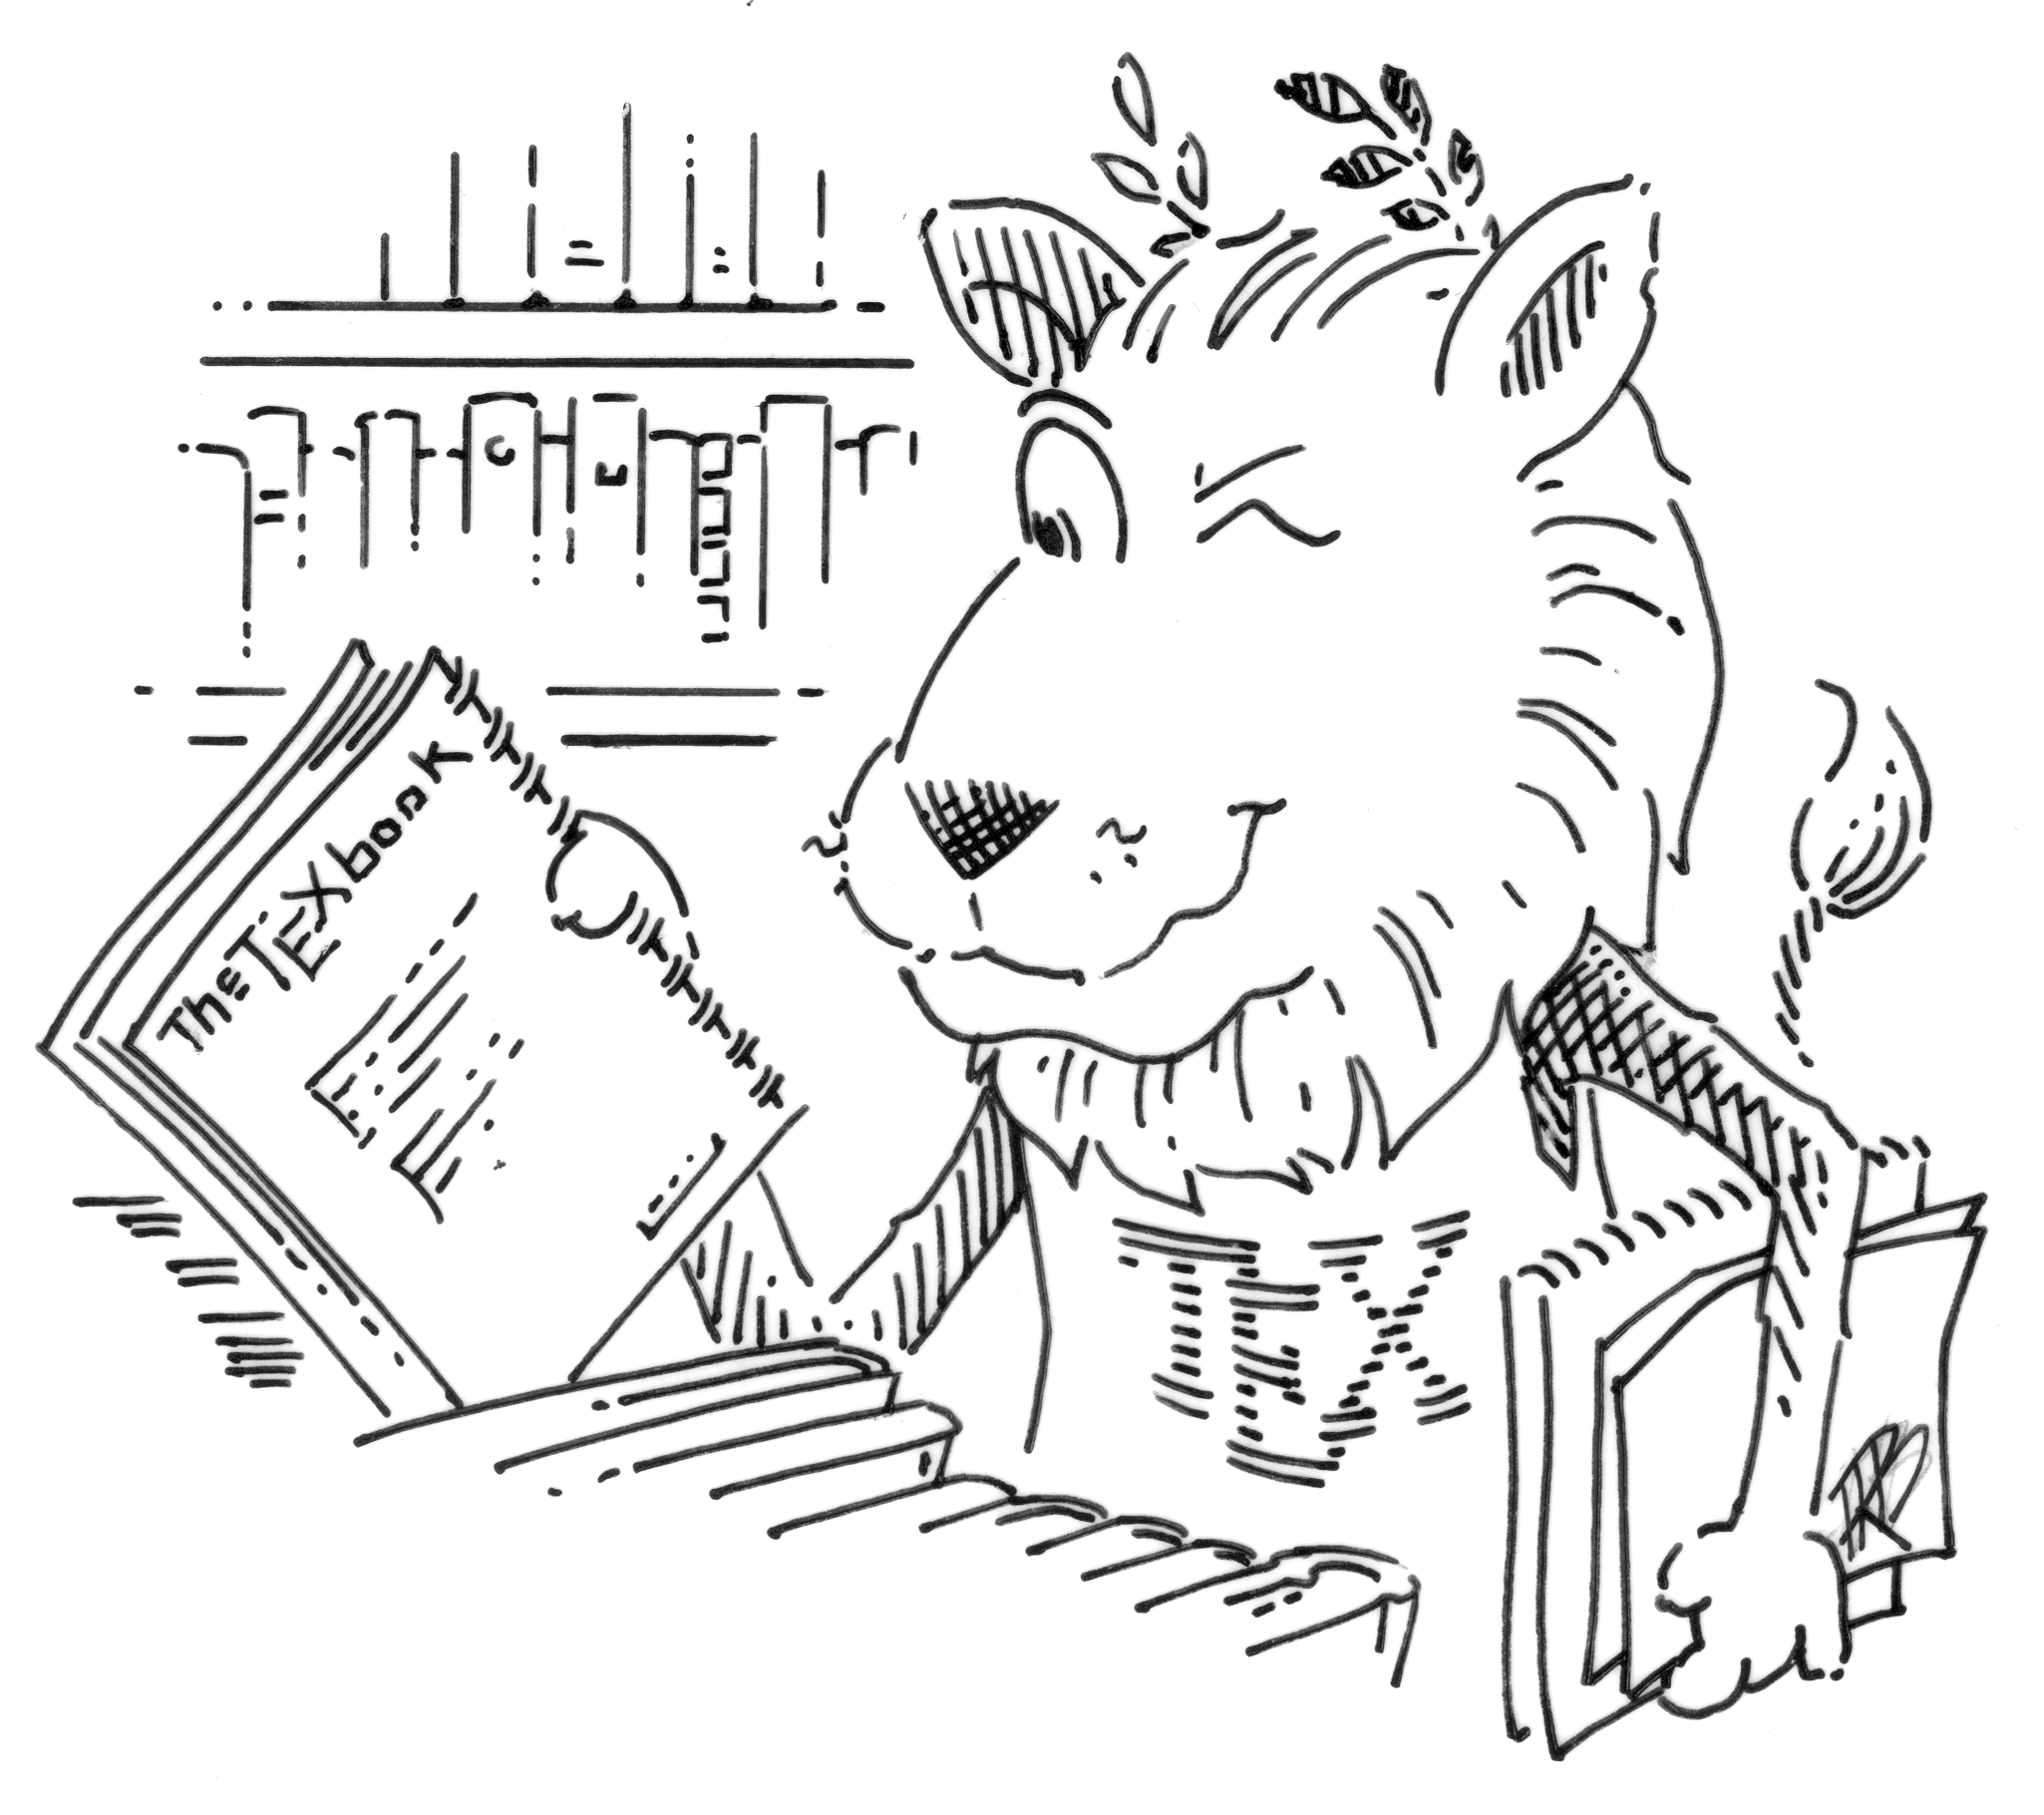
\includegraphics[width=1.5cm]{logo.jpg}
\end{minipage}
}
\usepackage{xepersian}
\title{یک نوشته نمونه}
\author{وفا خلیقی}
\author{مهدی امیدعلی}
\author{محمود امین‌طوسی}
\translator{وفا خلیقی}
\curraddr{ایران، مشهد، دانشگاه فردوسی}
\curraddr{ایران، مشهد، دانشگاه فردوسی}
\curraddr{ایران، مشهد، دانشگاه فردوسی}
\urladdr{http://um.ac.ir/~myhomepage}
\urladdr{http://um.ac.ir/~myhomepage}
\urladdr{http://um.ac.ir/~myhomepage}
\email{example@somedomain.com}
\email{mehdioa@gmail.com}
\email{m.amintoosi@gmail.com}
\dedicatory{تقدیم به جمشید کاشانی، ریاضی‌دان هموطنم}
\date{\today}
\copyrightinfo{1390}{(وفا خلیقی)}
\keywords{اعداد مرکب، نظریه رسته‌ها}
\thanks{از انجمن ریاضی ایران بابت حمایت‌هاشان تشکر می‌کنم}
\subjclass[2010]{Analysis; topology}
\begin{document}
\begin{abstract}
زمان تقریبی برای اتمام مرحله اول: مرحله اول شامل بنای زیرساختار سیمرغ است که شامل ماکروهای ساختاری تک و لوا می‌باشد (ماکروهای زیرساختاری لازم برای برنامه‌نویسی، حروف‌چینی راست به چپ، کشیدگی، قواعد نگارش زبان پارسی، الگوریتم حروف‌چینی دوجهته یونیکد و ...) که حدود ۳ سال طول می‌کشد.
\end{abstract}
\maketitle
\tableofcontents
\specialsection{موارد پیش‌بینی شده}
زمان تقریبی برای اتمام مرحله اول: مرحله اول شامل بنای زیرساختار سیمرغ است که شامل ماکروهای ساختاری تک و لوا می‌باشد (ماکروهای زیرساختاری لازم برای برنامه‌نویسی، حروف‌چینی راست به چپ، کشیدگی، قواعد نگارش زبان پارسی، الگوریتم حروف‌چینی دوجهته یونیکد و ...) که حدود ۳ سال طول می‌کشد. 
\begin{enumerate}
\item
یک
\item
دو
\end{enumerate}
\begin{equation}
1+2=3
\end{equation}
\section{مقدمه}
\newpage

این ادامه متن است
\setLTRbibitems
\begin{thebibliography}{99}%
\resetlatinfont

\bibitem{bgilkeyns}
 N.~Bla\v{z}i\'c, P.~Gilkey, S.~Nik\v{c}evi\'c, and U.~Simon, {\em
  Algebraic theory of affine curvature tensors}, Archivum Mathematicum, 42
  (2006), pp.~147--168.

\bibitem{chen}
 B.~Y. Chen and S.~W. Wei, {\em Differential geometry of submanifolds of
  warped product manifolds {$I\times_fS^{m-1}(k)$}}, J. Geom., 91 (2009),
  pp.~21--42.

\bibitem{onil2}
 B.~O`Neill, {\em Semi-{Riemannian geometry}}, Academic Press, 1986.

\bibitem{oprea}
 J.~Oprea, {\em Differential geometry and its applications}, Prentice
  Hall, second~ed., 2004.

\end{thebibliography}
\end{document}